%% Tratto da: https://www.researchgate.net/publication/228340819_Multilayer_perceptron_and_neural_networks
\section{Multi Layer Perceptron}
The Multi Layer Perceptron model is the most known and
most frequently used type of neural network. The signals are transmitted within the
network in one direction, from input to output: there
is no loop, the output of each neuron does not affect
the neuron itself.
Layers which are not directly connected to the
environment are called hidden.

There are also
feed-back networks, which can transmit impulses in
both directions, due to reaction connections in the
network. These types of networks are very powerful
and can be extremely complicated.
Introduction of several layers was
determined by the need to increase the complexity of
decision regions.

A perceptron with a single layer and one
input generates decision regions under the form of
semi planes. By adding another layer, each neuron
acts as a standard perceptron for the outputs of the
neurons in the anterior layer, thus the output of the
network can estimate convex decision regions,
resulting from the intersection of the semi planes
generated by the neurons.

The power of the multilayer perceptron comes
precisely from non-linear activation functions.
Almost any non-linear function can be used for this
purpose, except for polynomial functions. Currently,
the functions most commonly used today are the
single-pole (or logistic) sigmoid \cite{mlp}.

%% @VP meglio una sotto l'altra o disposte affiancate ?
\begin{figure}[H]
	\centering
	\begin{tikzpicture}
		\draw[->] (-5,0) -- (5,0) node[right] {$x$};
		\draw[->] (0,-2.1) -- (0,2.1) node[above] {$y$};
		\draw[dotted] (-5,-2.1) grid (5,2.1);
		\draw[color=blue] plot[id=logistic] function{1/(1+exp(-x))};
	\end{tikzpicture}
	\caption{Sigmoid function $\sigma(x) = \frac{1}{1+e^{-x}}$}
	\label{fig:sigmoid}
\end{figure}

\begin{figure}[H]
	\centering

	\tikzset{%
		every neuron/.style={
				circle,
				draw,
				minimum size=1cm
			},
		neuron missing/.style={
				draw=none,
				scale=4,
				text height=0.333cm,
				execute at begin node=\color{black}$\vdots$
			},
	}
	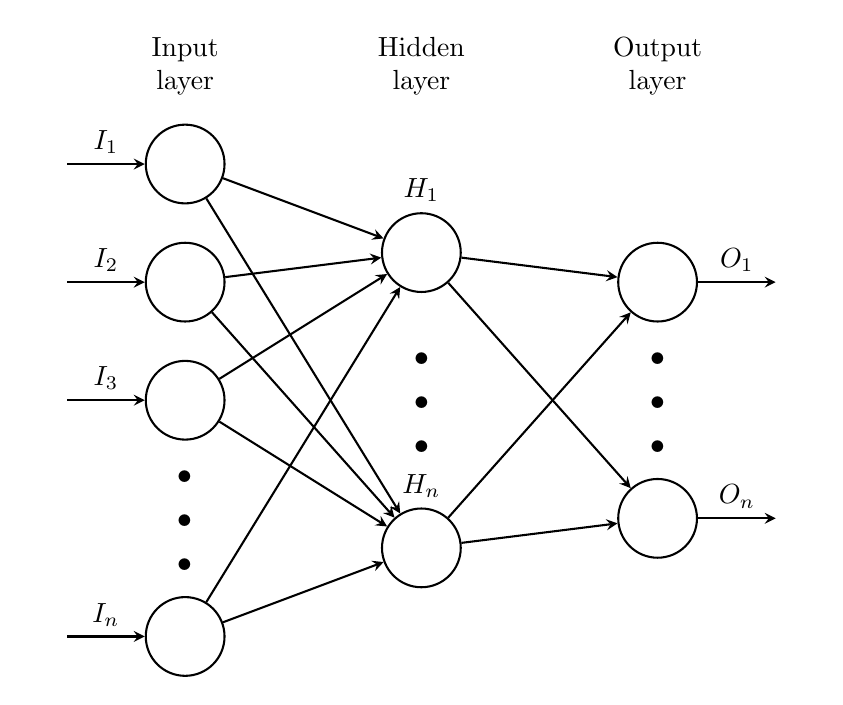
\begin{tikzpicture}[x=1.5cm, y=1.5cm, >=stealth]
		\foreach \m/\l [count=\y] in {1,2,3,missing,4}
		\node [every neuron/.try, neuron \m/.try] (input-\m) at (0,2.5-\y) {};

		\foreach \m [count=\y] in {1,missing,2}
		\node [every neuron/.try, neuron \m/.try ] (hidden-\m) at (2,2-\y*1.25) {};

		\foreach \m [count=\y] in {1,missing,2}
		\node [every neuron/.try, neuron \m/.try ] (output-\m) at (4,1.5-\y) {};

		\foreach \l [count=\i] in {1,2,3,n}
		\draw [<-] (input-\i) -- ++(-1,0)
		node [above, midway] {$I_\l$};

		\foreach \l [count=\i] in {1,n}
		\node [above] at (hidden-\i.north) {$H_\l$};

		\foreach \l [count=\i] in {1,n}
		\draw [->] (output-\i) -- ++(1,0)
		node [above, midway] {$O_\l$};

		\foreach \i in {1,...,4}
		\foreach \j in {1,...,2}
		\draw [->] (input-\i) -- (hidden-\j);

		\foreach \i in {1,...,2}
		\foreach \j in {1,...,2}
		\draw [->] (hidden-\i) -- (output-\j);

		\foreach \l [count=\x from 0] in {Input, Hidden, Output}
		\node [align=center, above] at (\x*2,2) {\l \\ layer};
	\end{tikzpicture}
	\caption{Multi Layer Perceprton architecture.}
	\label{fig:mlp-arch}
\end{figure}

%% Tratto da: https://arxiv.org/pdf/1912.05911.pdf
\section{Recurrent Neural Network}
Recurrent Neural Networks (RNNs) are a type of neural network architecture which is mainly used
to detect patterns in sequences of data. Such data can be handwriting, genomes, text or numerical
time series which are often produced in industry settings (e.g. stock markets or sensors).
However, they are also applicable to images if these get respectively decomposed into a series of
patches and treated as a sequence. On a higher level, RNNs find applications in Language
Modelling and Generating Text, Speech Recognition, Generating Image Descriptions or Video Tagging.

What differentiates Recurrent Neural Networks from Multi-Layer Perceptrons (MLPs) and in general Feedforward Neural Networks is how information gets passed through the network. While
Feedforward Networks pass information through the network without cycles, the RNN has cycles and
transmits information back into itself \cite{rnn}. This enables them to extend the functionality of Feedforward
Networks to also take into account previous inputs $X_{0:t-1}$ and not only the current input $X_t$. This
difference is visualised on a high level in Figure \ref{fig:mlpvsrnn}. Note, that here the option of having multiple
hidden layers is aggregated to one Hidden Layer block H. This block can obviously be extended to
multiple hidden layers.

\begin{figure}[H]
	\centering

	\tikzset{every picture/.style={line width=0.75pt}} %set default line width to 0.75pt        

	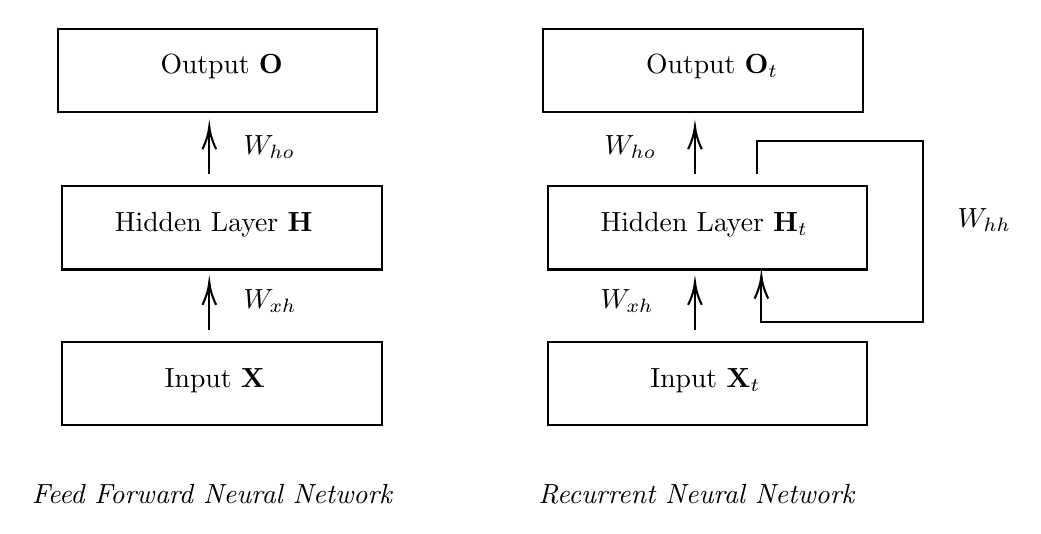
\begin{tikzpicture}[x=0.75pt,y=0.75pt,yscale=-1,xscale=1]
		%uncomment if require: \path (0,293); %set diagram left start at 0, and has height of 293

		%Shape: Rectangle [id:dp3269011808602339] 
		\draw   (177,166) -- (331,166) -- (331,206) -- (177,206) -- cycle ;

		%Shape: Rectangle [id:dp07456364437829421] 
		\draw   (177,91) -- (331,91) -- (331,131) -- (177,131) -- cycle ;

		%Shape: Rectangle [id:dp06593997739682389] 
		\draw   (175,15) -- (329,15) -- (329,55) -- (175,55) -- cycle ;

		%Straight Lines [id:da8268201466362239] 
		\draw    (248,160.1) -- (248,139.1) ;
		\draw [shift={(248,137.1)}, rotate = 90] [color={rgb, 255:red, 0; green, 0; blue, 0 }  ][line width=0.75]    (10.93,-3.29) .. controls (6.95,-1.4) and (3.31,-0.3) .. (0,0) .. controls (3.31,0.3) and (6.95,1.4) .. (10.93,3.29)   ;
		%Straight Lines [id:da37666922082080234] 
		\draw    (248,85.1) -- (248,64.1) ;
		\draw [shift={(248,62.1)}, rotate = 90] [color={rgb, 255:red, 0; green, 0; blue, 0 }  ][line width=0.75]    (10.93,-3.29) .. controls (6.95,-1.4) and (3.31,-0.3) .. (0,0) .. controls (3.31,0.3) and (6.95,1.4) .. (10.93,3.29)   ;
		%Shape: Rectangle [id:dp5633797539561046] 
		\draw   (411,166) -- (565,166) -- (565,206) -- (411,206) -- cycle ;

		%Shape: Rectangle [id:dp8965815577330951] 
		\draw   (411,91) -- (565,91) -- (565,131) -- (411,131) -- cycle ;

		%Shape: Rectangle [id:dp2829092094481056] 
		\draw   (409,15) -- (563,15) -- (563,55) -- (409,55) -- cycle ;

		%Straight Lines [id:da8493416258837974] 
		\draw    (482,160.1) -- (482,139.1) ;
		\draw [shift={(482,137.1)}, rotate = 90] [color={rgb, 255:red, 0; green, 0; blue, 0 }  ][line width=0.75]    (10.93,-3.29) .. controls (6.95,-1.4) and (3.31,-0.3) .. (0,0) .. controls (3.31,0.3) and (6.95,1.4) .. (10.93,3.29)   ;
		%Straight Lines [id:da4576582908562111] 
		\draw    (482,85.1) -- (482,64.1) ;
		\draw [shift={(482,62.1)}, rotate = 90] [color={rgb, 255:red, 0; green, 0; blue, 0 }  ][line width=0.75]    (10.93,-3.29) .. controls (6.95,-1.4) and (3.31,-0.3) .. (0,0) .. controls (3.31,0.3) and (6.95,1.4) .. (10.93,3.29)   ;
		%Straight Lines [id:da05080047786173725] 
		\draw    (512,85.1) -- (512,69.1) -- (592,69.1) -- (592,156.1) -- (514,156.1) -- (514,136.1) ;
		\draw [shift={(514,134.1)}, rotate = 90] [color={rgb, 255:red, 0; green, 0; blue, 0 }  ][line width=0.75]    (10.93,-3.29) .. controls (6.95,-1.4) and (3.31,-0.3) .. (0,0) .. controls (3.31,0.3) and (6.95,1.4) .. (10.93,3.29)   ;

		% Text Node
		\draw (223,26) node [anchor=north west][inner sep=0.75pt]   [align=left] {Output \textbf{O}};
		% Text Node
		\draw (225,177) node [anchor=north west][inner sep=0.75pt]   [align=left] {Input \textbf{X}};
		% Text Node
		\draw (201,102) node [anchor=north west][inner sep=0.75pt]   [align=left] {Hidden Layer \textbf{H}};
		% Text Node
		\draw (263,139) node [anchor=north west][inner sep=0.75pt]   [align=left] {$\displaystyle W_{xh}$};
		% Text Node
		\draw (263,65) node [anchor=north west][inner sep=0.75pt]   [align=left] {$\displaystyle W_{ho}$};
		% Text Node
		\draw (435,139) node [anchor=north west][inner sep=0.75pt]   [align=left] {$\displaystyle W_{xh}$};
		% Text Node
		\draw (437,65) node [anchor=north west][inner sep=0.75pt]   [align=left] {$\displaystyle W_{ho}$};
		% Text Node
		\draw (457,26) node [anchor=north west][inner sep=0.75pt]   [align=left] {Output \textbf{O}$\displaystyle _{t}$};
		% Text Node
		\draw (435,102) node [anchor=north west][inner sep=0.75pt]   [align=left] {Hidden Layer \textbf{H}$\displaystyle _{t}$};
		% Text Node
		\draw (459,177) node [anchor=north west][inner sep=0.75pt]   [align=left] {Input \textbf{X}$\displaystyle _{t}$};
		% Text Node
		\draw (607,100) node [anchor=north west][inner sep=0.75pt]   [align=left] {$\displaystyle W_{hh}$};
		% Text Node
		\draw (161,233) node [anchor=north west][inner sep=0.75pt]   [align=left] {\textit{Feed Forward Neural Network}};
		% Text Node
		\draw (405,233) node [anchor=north west][inner sep=0.75pt]   [align=left] {\textit{Recurrent Neural Network}};


	\end{tikzpicture}

	\caption{Visualization of difference between MLPs and RNN.}
	\label{fig:mlpvsrnn}
\end{figure}

%% @VP come si calcola l'output e i pesi ce lo metto (formule matematiche)?

% Tratto da: https://datascience.eu/machine-learning/gated-recurrent-units-understanding-the-fundamentals/
% Paper dove sono state introdotte: https://arxiv.org/abs/1406.1078
\subsection{Gated Recurrent Unit}
Gated Recurrent Units (GRU) are an advanced variation of RRNs (Recurrent Neural Network) \cite{gru2}.
GRUs use update gate and reset get for solving a standard RNN’s vanishing gradient issue. These are essentially 2 vectors that decide the type of information to be passed towards the output. What makes these vectors special is that programmers can train them to store information, especially from long ago \cite{gru1}.

They do all of this by utilizing its gated units which help solve vanishing/exploding gradient problems often found in traditional recurrent neural networks. These gates are helpful for controlling any information to be maintained or discarded for each step. It is also worth keeping in mind that gated recurrent units make use of reset and update gates.

\begin{itemize}
	\item \textbf{Update Gate’s Function}: The main function of the update gate is to determine the ideal amount of earlier info that is important for the future. One of the main reasons why this function is so important is that the model can copy every single past detail to eliminate fading gradient issue.
	\item \textbf{Reset Gate's Function}: A major reason why reset gate is vital because it determines how much information should be ignored. It would be fair to compare reset gate to LSTM’s forget gate because it tends to classify unrelated data, followed by getting the model to ignore and proceed without it.
\end{itemize}

\begin{figure}[H]
	\centering
	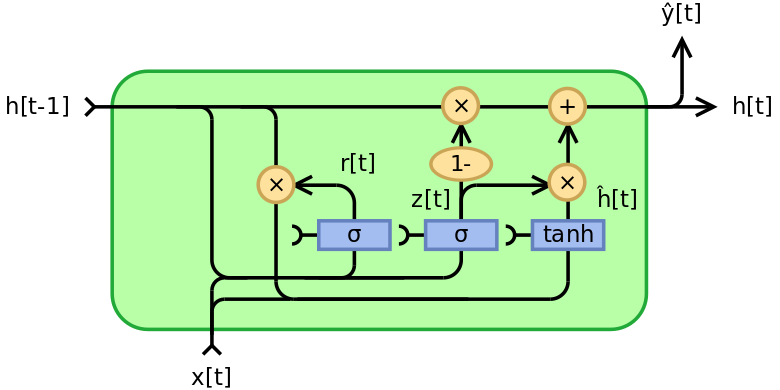
\includegraphics[width=.90\linewidth]{chapters/1_introduction/imgs/gru.png}
	\caption{Gated Recurrent Unit (GRU) architecture.}
	\label{fig:gruarch}
\end{figure}

%% Tratto da: https://arxiv.org/pdf/1706.03762.pdf
\section{Transformer}

Recurrent neural networks, long short-term memory and gated recurrent neural networks
in particular, have been firmly established as state of the art approaches in sequence modeling and
transduction problems such as language modeling and machine translation \cite{trans2}.
Recurrent models typically factor computation along the symbol positions of the input and output
sequences. Aligning the positions to steps in computation time, they generate a sequence of hidden
states $h_t$, as a function of the previous hidden state $h_{t-1}$
and the input for position $t$. This inherently
sequential nature precludes parallelization within training examples, which becomes critical at longer
sequence lengths, as memory constraints limit batching across examples.
Attention mechanisms \cite{attention} have become an integral part of compelling sequence modeling and transduction models in various tasks, allowing modeling of dependencies without regard to their distance in
the input or output sequences.
The Transformer allows for significantly more parallelization \cite{trans1}.

\begin{figure}[H]
	\centering
	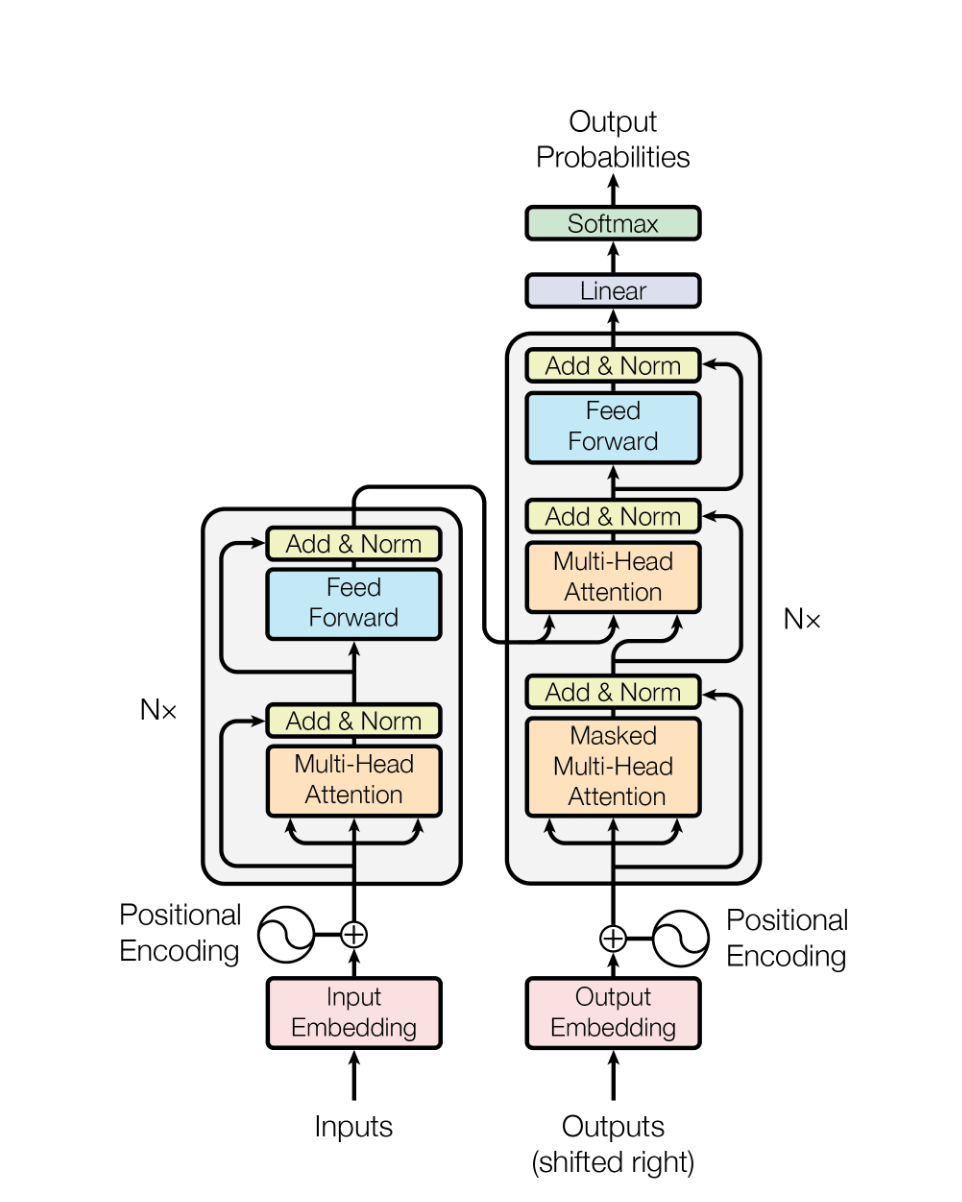
\includegraphics[width=10cm, keepaspectratio]{chapters/1_introduction/imgs/transformers.png}
	\caption{This figure shows the Transformers model architecture \cite{attention}.}
	\label{fig:transarch}
\end{figure}

Most competitive neural sequence transduction models have an encoder-decoder structure \cite{trans2}.
Here, the encoder maps an input sequence of symbol representations $(x_1, \ldots, x_n)$ to a sequence
of continuous representations $z = (z_1, \ldots, z_n)$. Given $z$, the decoder then generates an output
sequence $(y_1, \ldots, y_m)$ of symbols, one element at a time. At each step the model is auto-regressive, consuming the previously generated symbols as additional input when generating the next.

The Transformer follows this overall architecture using stacked self-attention and point-wise, fully
connected layers for both the encoder and decoder, shown in the left and right halves of Figure \ref{fig:transarch}, respectively.

\begin{itemize}
	\item \textit{Encoder}: The encoder is composed of a stack of $N = 6$
	      identical layers. Each layer has two
	      sub-layers. The first is a multi-head self-attention mechanism\cite{attention}, and the second is a simple, position-
	      wise fully connected feed-forward network. Residual connection
	      are employed around each of
	      the two sub-layers, followed by layer normalization. That is, the output of each sub-layer is
	      $\text{LayerNorm}(x + \text{Sublayer}(x))$, where $\text{Sublayer}(x)$ is the function implemented by the sub-layer
	      itself. To facilitate these residual connections, all sub-layers in the model, as well as the embedding
	      layers, produce outputs of dimension $dmodel = 512$.

	\item \textit{Decoder}: The decoder is also composed of a stack of $N = 6$
	      identical layers. In addition to the two
	      sub-layers in each encoder layer, the decoder inserts a third sub-layer, which performs multi-head
	      attention over the output of the encoder stack. Similar to the encoder, there are residual connections
	      around each of the sub-layers, followed by layer normalization. The self-attention sub-layer is modified in the decoder stack to prevent positions from attending to subsequent positions. This
	      masking\cite{attention}, combined with fact that the output embeddings are offset by one position, ensures that the
	      predictions for position $i$ can depend only on the known outputs at positions less than $i$.

	\item \textit{Attention}: An attention\cite{attention} function can be described as
	      mapping a query and a set of key-value pairs to an output,
	      where the query, keys, values, and output are all vectors\cite{trans1}. The output is computed as a weighted sum of the values, where the weight assigned to each value is computed by a compatibility function of the
	      query with the corresponding key\cite{attention}.
\end{itemize}

\begin{figure}[H]
	\centering
	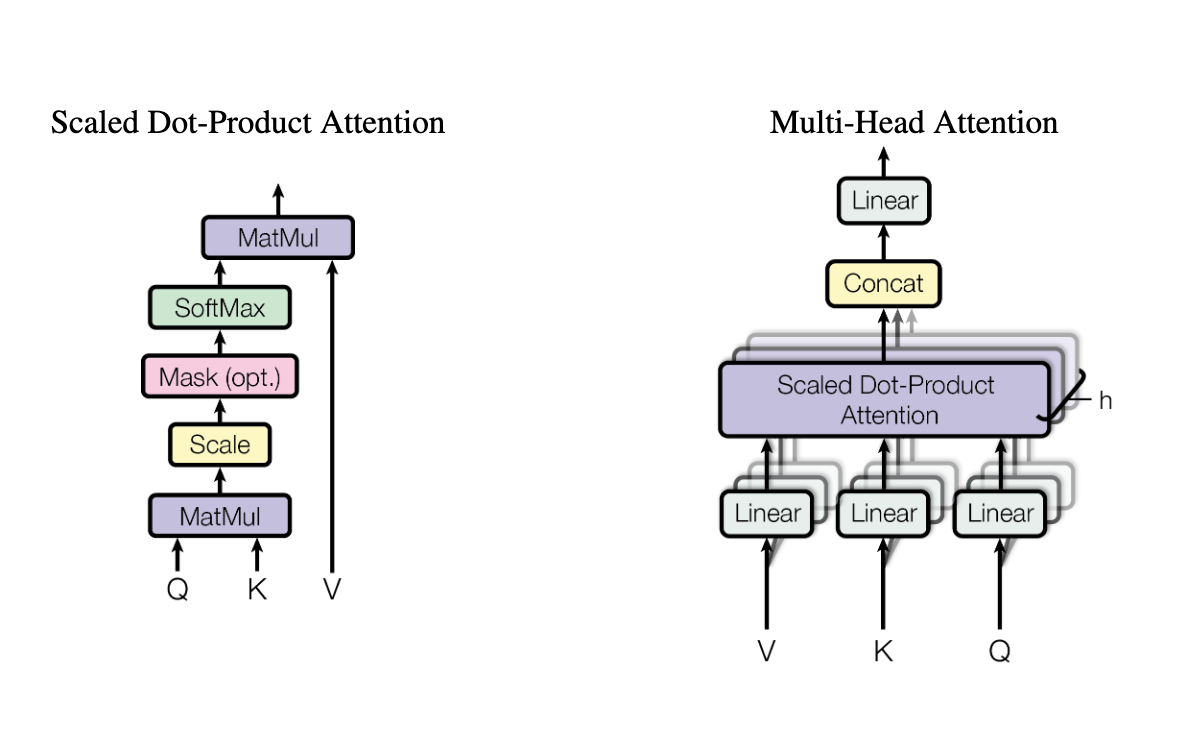
\includegraphics[width=12cm, keepaspectratio]{chapters/1_introduction/imgs/attention.png}
	\caption{Scaled Dot-Product Attention\cite{attention} (left). Multi-Head Attention\cite{attention} consists of several attention layers running in parallel (right).}
	\label{fig:attention}
\end{figure}
%
%%% Immagine di Optimus Prime, un Transformer
%%%      ce lo mettiamo ??
%%\begin{figure}
%%    \centering
%%    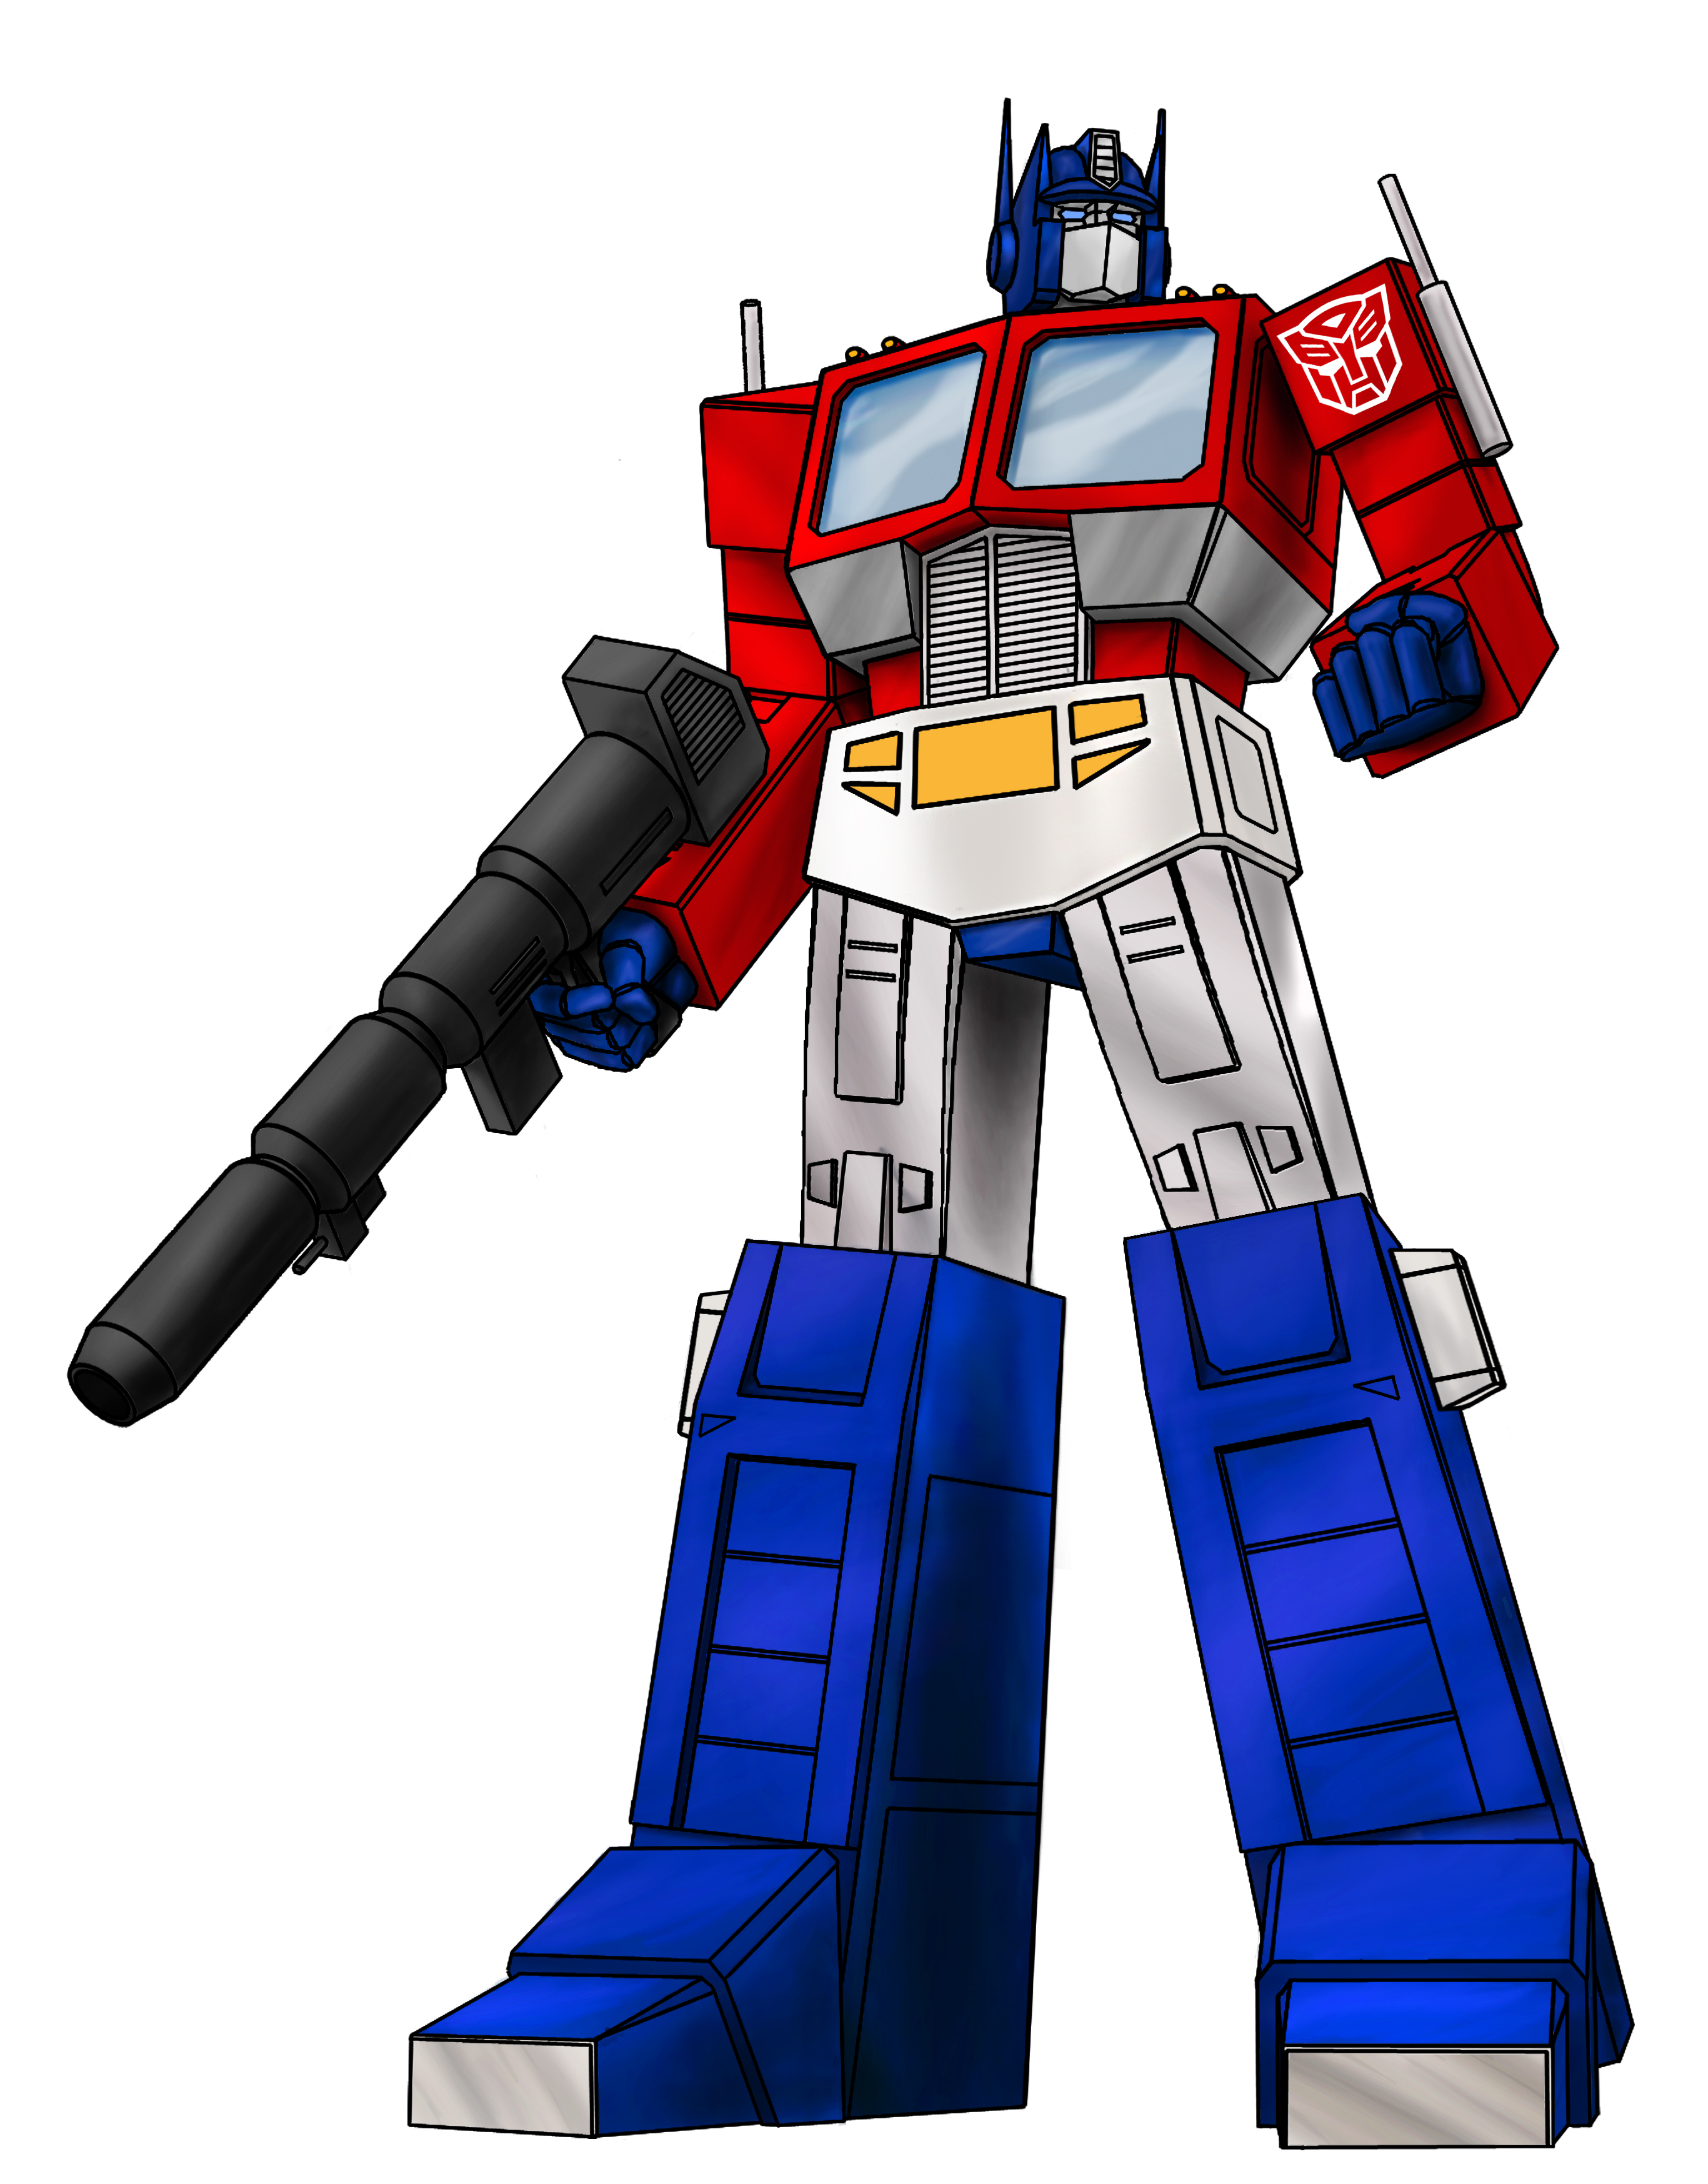
\includegraphics[width=0.5\linewidth]{chapters/1_introduction/imgs/optimusprime.png}
%%    \caption{Enter Caption}
%%    \label{fig:enter-label}
%%\end{figure}